\documentclass[oneside,a4paper,14pt]{extarticle} %размер шрифта 14
\usepackage[T1,T2A]{fontenc}
\usepackage[
a4paper,
letterpaper,
top=2cm,
bottom=2cm,
left=2.5cm,
right=1.5cm
]{geometry}
\usepackage[utf8]{inputenc} %кодировка текста
\usepackage[russian]{babel} %поддержка русского языка
\usepackage{textcomp} %текстовые символы
\usepackage{indentfirst} %корректировка отступов
\usepackage{listings} %для кода !!
\usepackage{xcolor}
% \usepackage{minted} %для кода !!!
\usepackage{enumitem} %для нумерации буквами
\usepackage{graphicx} %работа с изображениям
\usepackage{mwe} % for blindtext and example-image-a in example
\usepackage{wrapfig}
\usepackage{caption}
\usepackage{amsmath}  % для формул и символов
\usepackage{amsfonts}
\usepackage{float}
\usepackage{amsthm}
\usepackage{graphicx}
\usepackage[all]{xy}
\usepackage[breaklinks]{hyperref}
%%размеркегляузаголоковразделов
\usepackage{titlesec}
\titleformat{\section}
{\normalsize\bfseries}
{\thesection} {1em}{}
\titleformat{\subsection}
{\normalsize\bfseries}
{\thesubsection} {1em}{}
\titleformat{\subsubsection}
{\normalsize\bfseries}
{\thesubsection} {1em}{}

\renewcommand\baselinestretch{1.33}\normalsize % межстрочный интервал
\setlength{\parindent}{1.25cm}
\usepackage{indentfirst}

% \setminted{fontsize=\small}
\lstset{
	language=C,
	basicstyle=\ttfamily\small,
	keywordstyle=\color{blue},
	commentstyle=\color{green!60!black},
	stringstyle=\color{red},
	numbers=left,
	numberstyle=\tiny\color{gray},
	frame=single,
	breaklines=true,
	showstringspaces=false,
	tabsize=2,
	inputencoding=utf8,
	extendedchars=true
}

\begin{document}
	\newpage\thispagestyle{empty}
	\begin{center}
		МИНИСТЕРСТВО НАУКИ И ВЫСШЕГО ОБРАЗОВАНИЯ\\
		РОССИЙСКОЙ ФЕДЕРАЦИИ
		ФЕДЕРАЛЬНОЕ ГОСУДАРСТВЕННОЕ БЮДЖЕТНОЕ\\
		ОБРАЗОВАТЕЛЬНОЕ
		УЧРЕЖДЕНИЕ ВЫСШЕГО ОБРАЗОВАНИЯ\\
		«ВЯТСКИЙ ГОСУДАРСТВЕННЫЙ УНИВЕРСИТЕТ»\\
		Институт математики и информационных систем\\
		Факультет автоматики и вычислительной техники\\
		Кафедра электронных вычислительных машин
	\end{center}
	\vspace{20mm}
	
	\begin{center}
		Отчёт по лабораторной работе №1\\
		по дисциплине\\
		<<Алгоритмы и структуры данных>>\\
	\end{center}
	\vspace{48mm}
	
	\noindent
	Выполнил студент гр. ИВТб-1303-06-00 \hfill \rule[-0,5mm]{30mm}{0.15mm}\,/Шубин В. Ю./
	\newline
	Проверил заведующий кафедрой ЭВМ \hfill \rule[-0,5mm]{30mm}{0.15mm}\,/Долженкова М.Л./
	
	\vfill
	\begin{center}
		Киров\\
		2026
	\end{center}
	
	\newpage
	\thispagestyle{empty}
	
	\section*{Цель работы:} формирование навыков алгоритмического мышления посредством решения набора задач с предопределенными характеристиками и уровнем сложности.
	\section*{Номера заданий:}
	\begin{enumerate}
		\item https://codeforces.com/contest/1656/problem/B
		\item https://codeforces.com/contest/1689/problem/B
		\item https://codeforces.com/contest/1165/problem/B
	\end{enumerate}
	\noindent Ссылка на профиль пользователя:\\
	\indent https://codeforces.com/profile/shubeeeert \\
	\noindent Ссылки на отправления:
	\begin{enumerate}
		\item https://codeforces.com/contest/1656/submission/373596289
		\item https://codeforces.com/contest/1689/submission/373597189
		\item https://codeforces.com/contest/1165/submission/377830318
	\end{enumerate}
	\newpage
	\section*{Решение заданий}
	\subsection*{Задание 1:}
\begin{figure}[H]
	\centering
	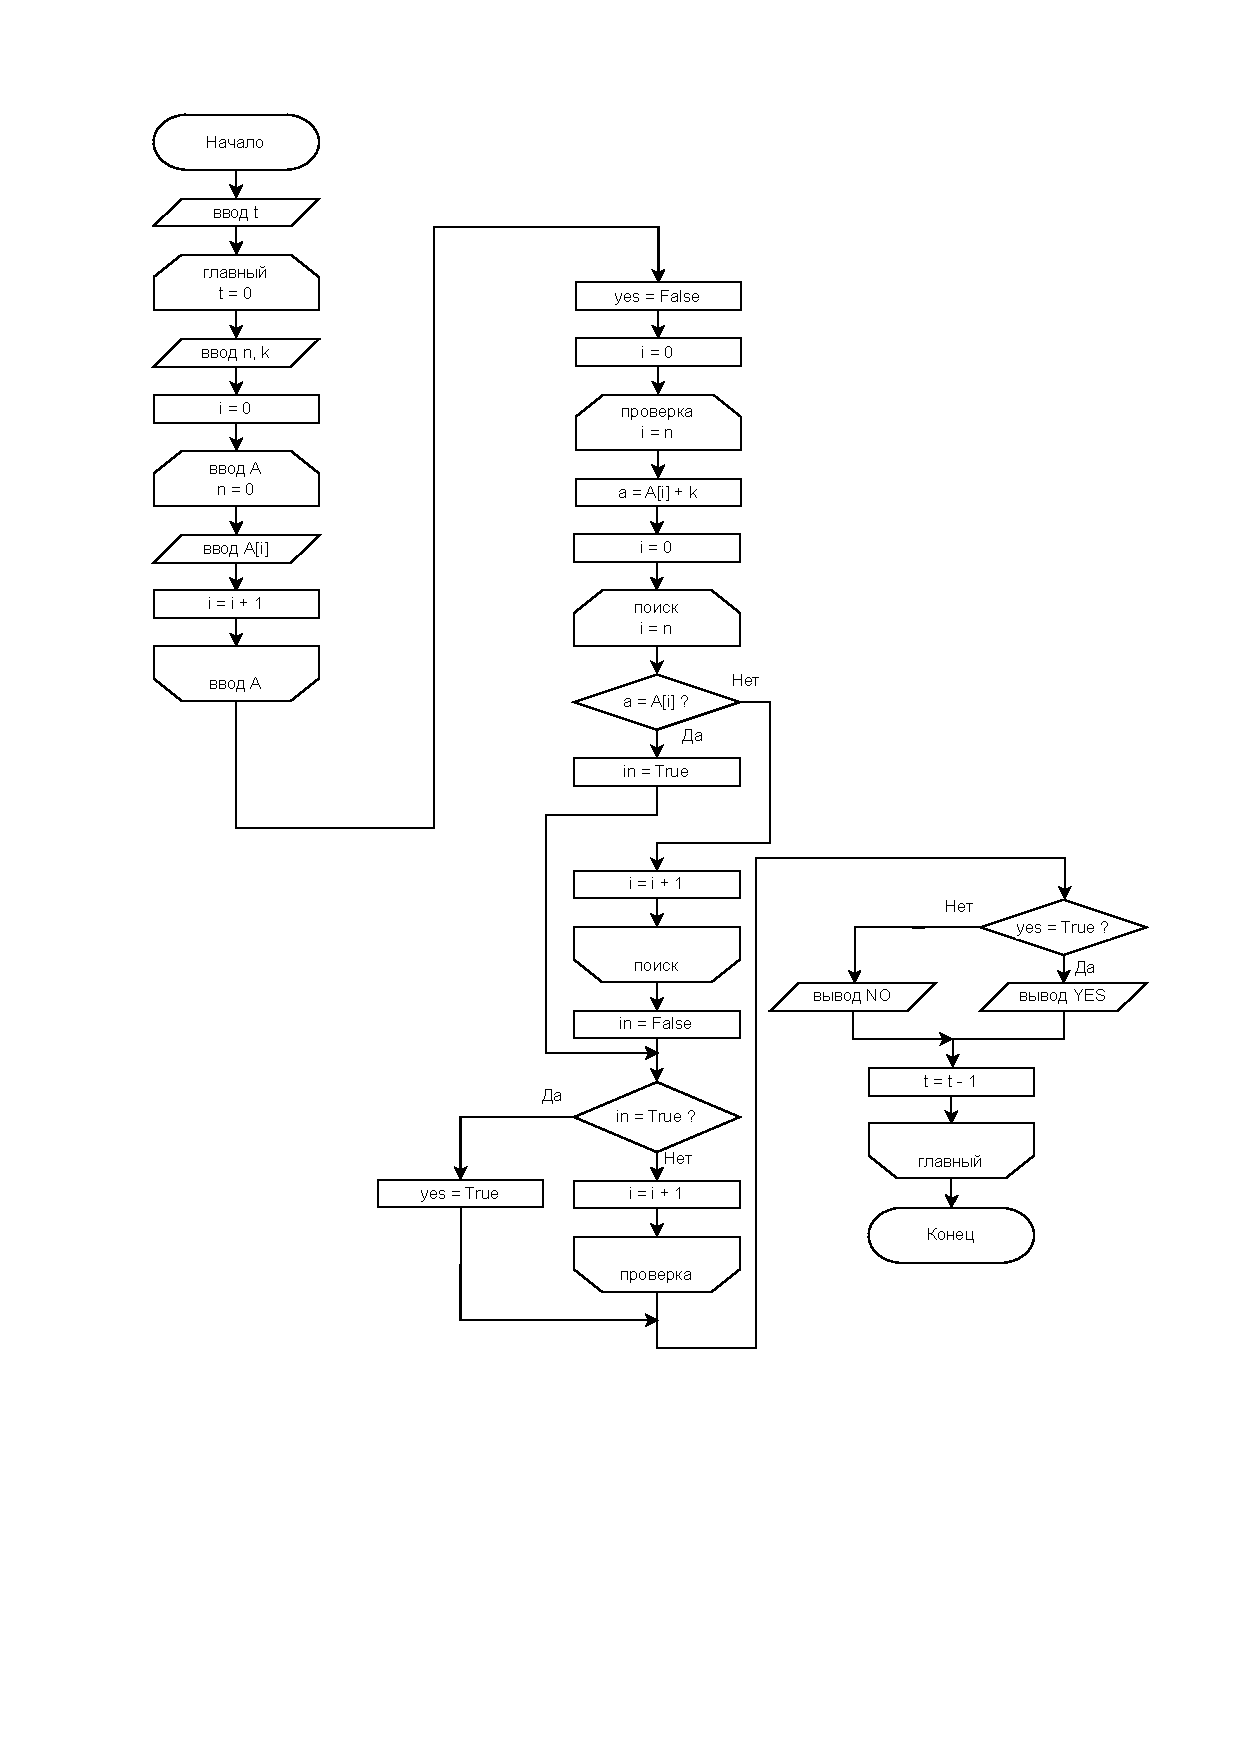
\includegraphics[width=\textwidth, height=0.9\textheight, keepaspectratio]{1.pdf}
	\caption{Схема алгоритма задачи}
\end{figure}
\lstinputlisting[caption={Исходный код программы (Python)}]{1.py}
\noindent \indent

Суть данного задания - проверить, есть ли в исходном массиве 2 числа, разность которых равна k. В коде это реализовано через цикл, 
проходящий по массиву, и сумму текущего числа с k.

\newpage
\subsection*{Задание 2:}
\begin{figure}[H]
	\centering
	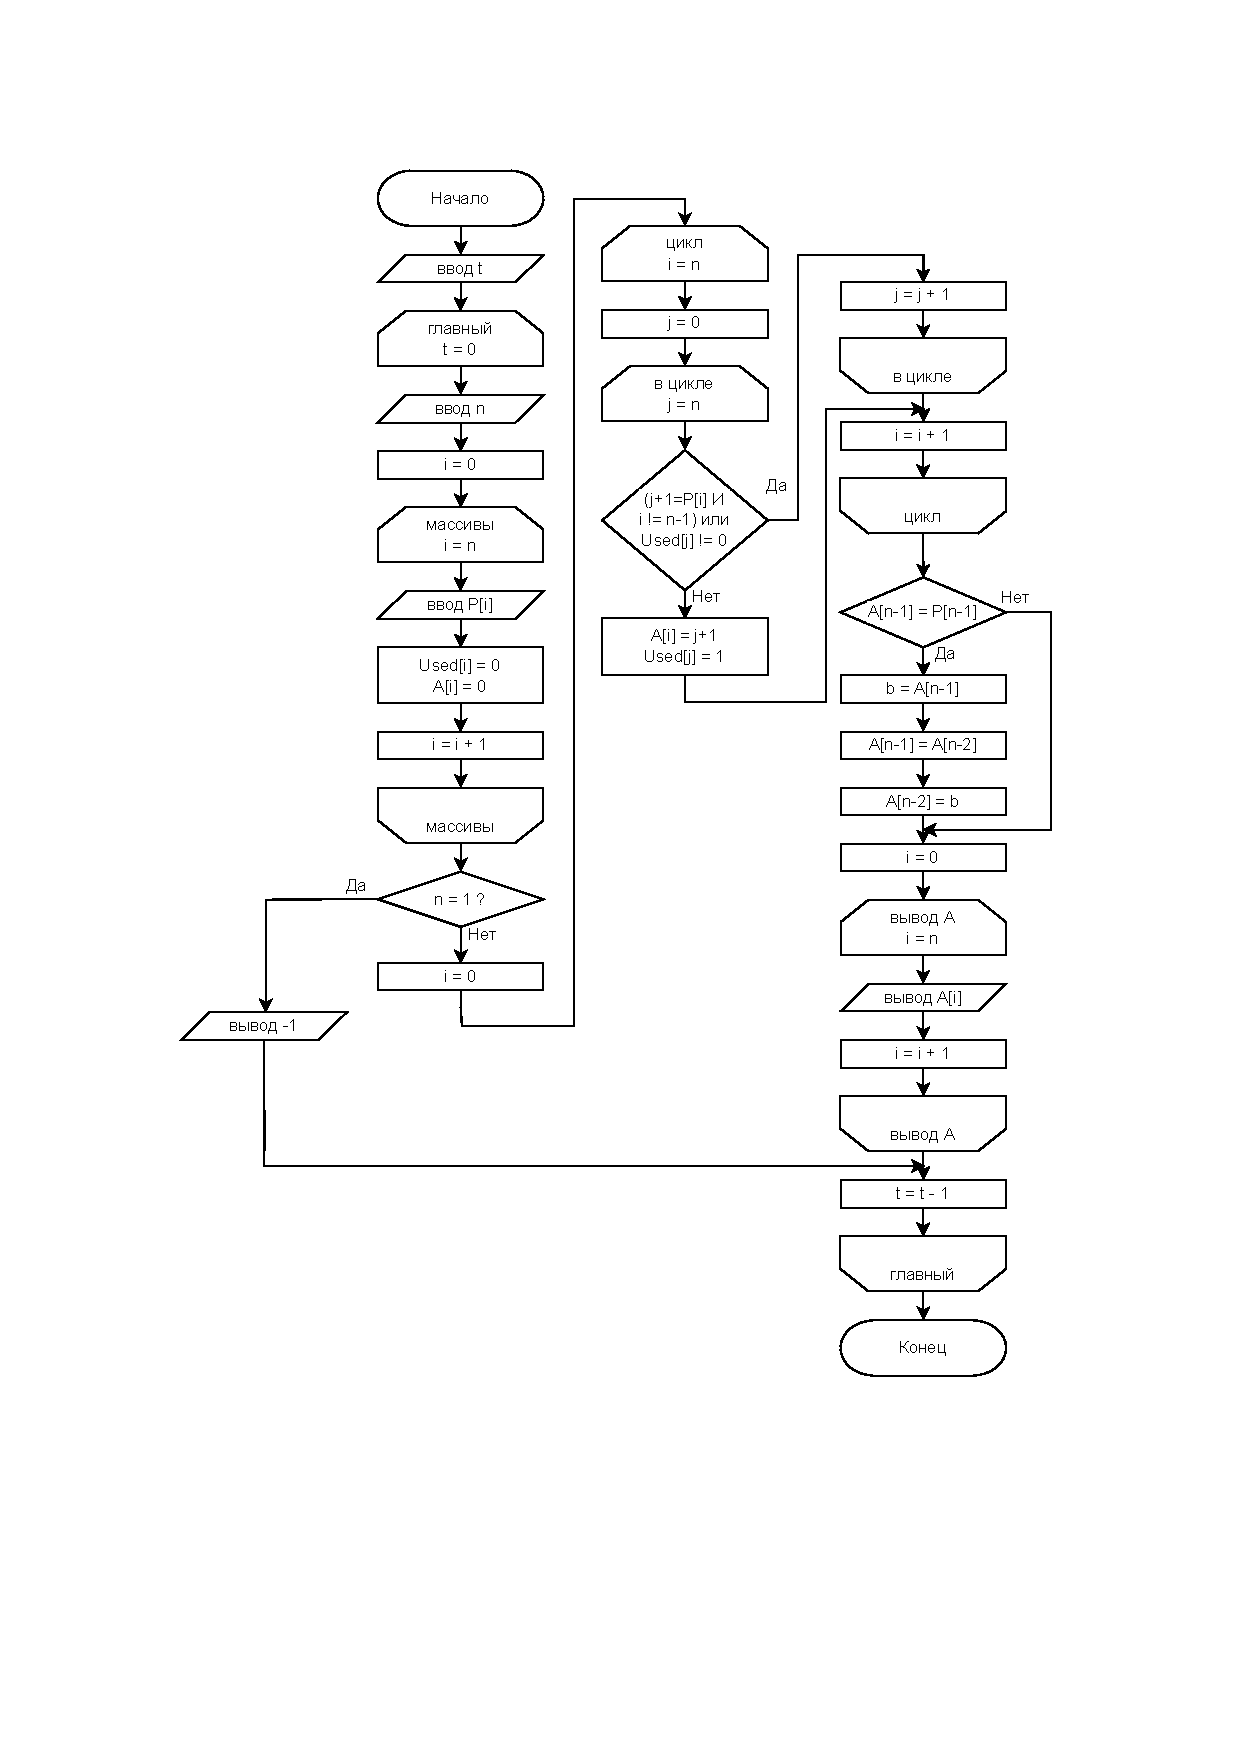
\includegraphics[width=\textwidth, height=0.9\textheight, keepaspectratio]{2.pdf}
	\caption{Схема алгоритма задачи}
\end{figure}
\newpage
\lstinputlisting[caption={Исходный код программы (Python)}]{3.py}
\noindent \indent

Суть данного задания - для каждой позиции пытаться подставить самое маленькое еще не использованное число, не совпадающее с число в этой позиции в исходном массиве.
Если совпадает, берем следующее по величине число. Для последнего числа проверяем, совпадает ли оно с числом из исходного массива - если да, меняем последнее и предпоследнее местами.

\newpage
\subsection*{Задание 3:}
\begin{figure}[H]
	\centering
	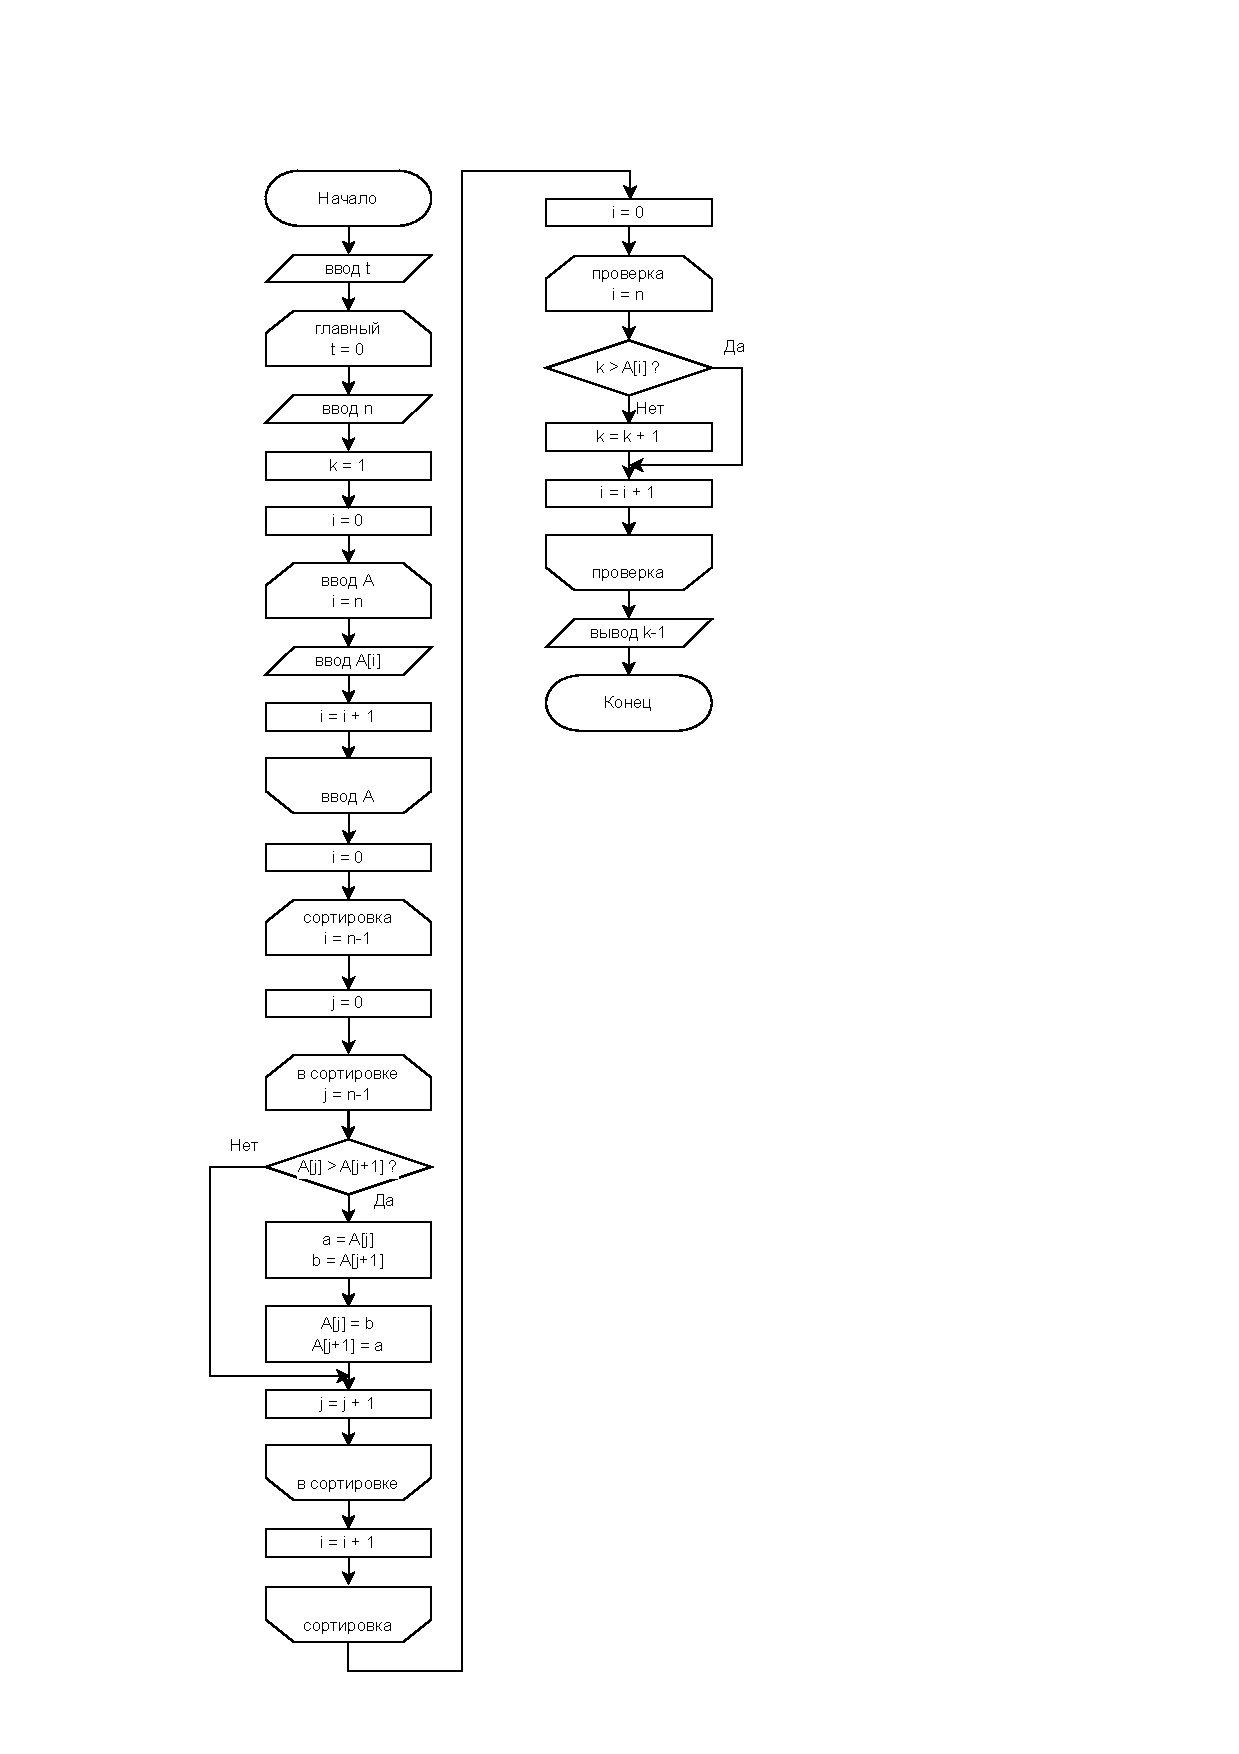
\includegraphics[width=\textwidth, height=0.9\textheight, keepaspectratio]{3.pdf}
	\caption{Схема алгоритма задачи}
\end{figure}
\newpage
\lstinputlisting[caption={Исходный код программы (Python)}]{3.py}
\noindent \indent

Суть данного задания - отсортировать массив по возрастанию и завести счетчик k для определения "текущего" дня по счету. Если в i-ый день кол-во контестов меньше k, пропускаем этот день,
В ином случае - увеличиваем k на 1 (т.е. переходим на следующий день решения контестов).

\newpage
	\section*{Выводы} Решение данных задач позволяет разобраться в простой оптимизации алгоритма,
	чтобы уложиться в жёсткий лимит по времени. Если пытаться решать эти задачи в лоб, как цикл в цикле или перебором,
	то ничего не получится. Для решения нужно заранее вычислять значения, чтобы приблизиться к $Q(n \cdot log(n))$ или даже $Q(n)$. 
	Думаю, главное, что мне пригодилось - не перебирать значения циклом в цикле, а находить какое-то необычное условие для быстрой проверки
	(например, в задаче 1, где нужно найти, есть ли в массиве два элемента с разностью k).
	Вообщем, для решения задач нужно не просто перебирать значения или "в лоб"\ решать, а надо оптимизировать кол-во повторений/проход в цикле,
	а также следует подбирать подходящие инструменты индивидуально для каждой задачи.
	
	
\end{document}